% Name: NFA for a regular expression
% Description: A four-state NFA for (a|b)*abb: it stays in q0 on any letter, then guesses where the final abb begins.
% Tags: NFA, regular expression, nondeterministic, regular language

\usetikzlibrary{automata, positioning}

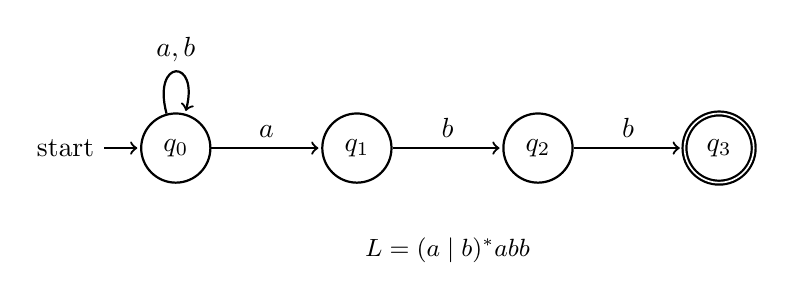
\begin{tikzpicture}[shorten >=1pt, node distance=2.3cm, on grid, auto, thick]
  \node[state, initial] (q0) {$q_0$};
  \node[state] (q1) [right=of q0] {$q_1$};
  \node[state] (q2) [right=of q1] {$q_2$};
  \node[state, accepting] (q3) [right=of q2] {$q_3$};

  \path[->]
    (q0) edge[loop above] node {$a, b$} ()
         edge node {$a$} (q1)
    (q1) edge node {$b$} (q2)
    (q2) edge node {$b$} (q3);
  \node[font=\small] at (3.45,-1.3) {$L = (a \mid b)^{*}abb$};
\end{tikzpicture}
